\mode*

% Since this a solution template for a generic talk, very little can
% be said about how it should be structured. However, the talk length
% of between 15min and 45min and the theme suggest that you stick to
% the following rules:  

% - Exactly two or three sections (other than the summary).
% - At *most* three subsections per section.
% - Talk about 30s to 2min per frame. So there should be between about
%   15 and 30 frames, all told.


\section{Logging}

\subsection{Securing Logging Mechanisms}

\begin{frame}
  \begin{example}
    \begin{itemize}
      \item Have a process write log messages to a file.
    \end{itemize}
  \end{example}

  \pause

  \begin{remark}
    \begin{itemize}
      \item Then the running process must access the file.
    \end{itemize}
  \end{remark}
\end{frame}

\begin{frame}
  \begin{solution}[Log internally]
    \begin{itemize}
      \item Could be done using append only access, thus no reading or 
        rewriting.
      \item Could trust the program but not the user.
      \item But only if the user doesn't have access to the hardware.
    \end{itemize}
  \end{solution}

  \pause

  \begin{question}
    \begin{itemize}
      \item How do we know if the user has managed to modify the logs?
    \end{itemize}
  \end{question}
\end{frame}

\begin{frame}
  \begin{solution}[Log externally]
    \begin{itemize}
      \item We could log to another system.
      \item This helps us if we don't trust the user or the process.
    \end{itemize}
  \end{solution}

  \pause

  \begin{remark}
    \begin{itemize}
      \item The problem remains with the sysadmin who has superuser access to 
        the external system.
    \end{itemize}
  \end{remark}
\end{frame}

\begin{frame}
  \begin{solution}[External with separation-of-duties]
    \begin{itemize}
      \item The sysadmin problem can be solved using a clever setup of 
        separation of duties.

      \item E.g.\ the logs of sysadmin \(A\) will be stored under the control of 
        sysadmins \(B\) and \(C\).

      \item This way sysadmin \(A\) can do everything except modify his own 
        logging mechanisms.

      \item The downside of this is that all systems must be online for this to 
        work.
    \end{itemize}
  \end{solution}
\end{frame}

\subsection{Schneier-Kelsey Logs}

\begin{frame}
  \begin{idea}[Schneier--Kelsey logs]
    \begin{itemize}
      \item Provides a secure logging mechanism for storing logs in an untrusted 
        machine.

      \item The untrusted machine is expected to work correctly up to a time 
        \(t\) when it is compromised by an attacker.

      \item The logs \(L_1, \ldots, L_{t-1}\) (before \(t\)) are provided with 
        confidentiality and integrity.
    \end{itemize}
  \end{idea}

  \pause

  \begin{remark}
    \begin{itemize}
      \item All logs \(L_t, L_{t+1}, \ldots\) generated from this point, however, 
        are under the influence of the attacker.

      \item The adversary can even delete them.
    \end{itemize}
  \end{remark}
\end{frame}

\begin{frame}
  \begin{figure}
    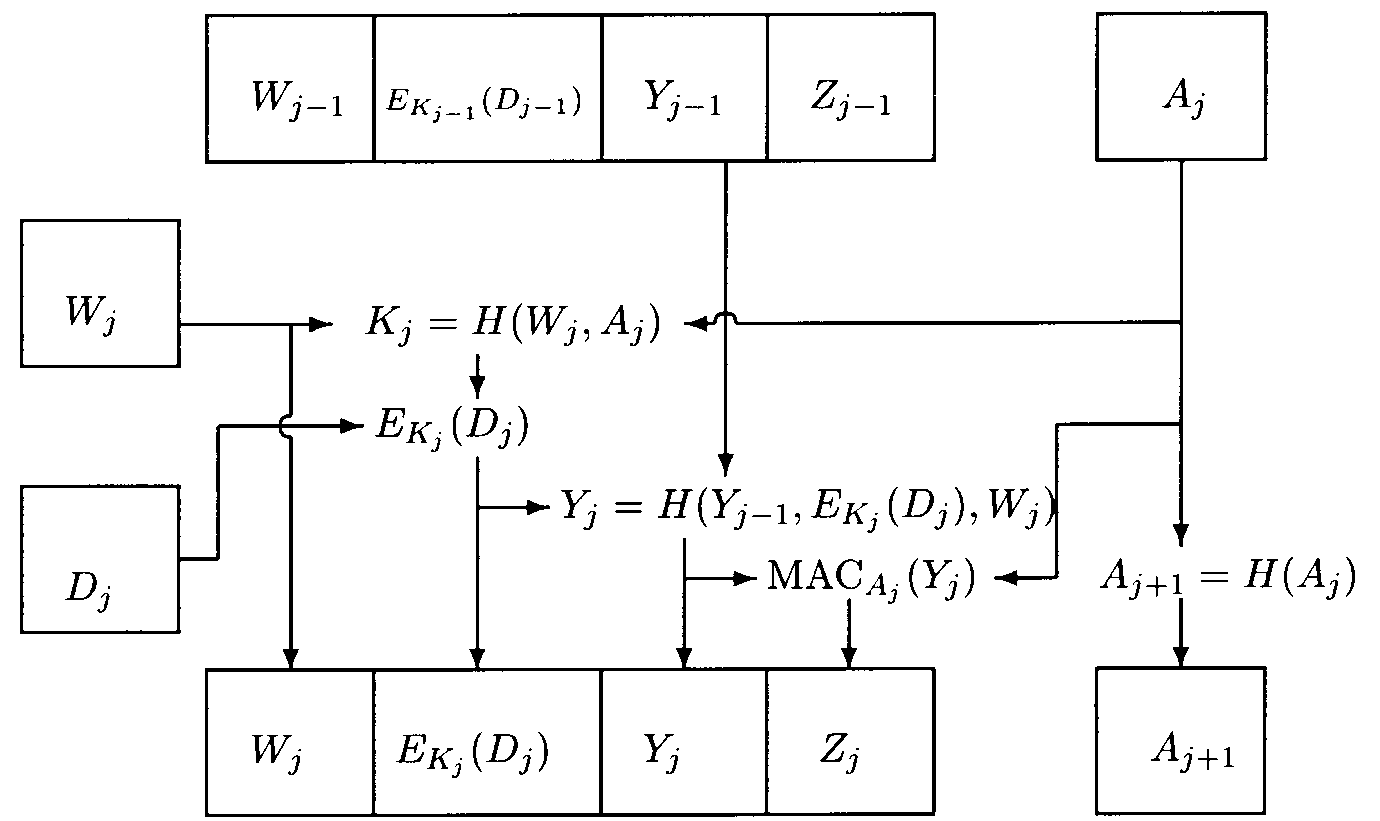
\includegraphics[height=0.7\textheight]{seclog.png}
    \caption{%
      Schneier-Kelsey secure-log scheme; \(W_j\) is the type of entry, \(D_j\) 
      is entry data, \(K_j\) is entry key, \(A_j\) is authentication key, and 
      \(H\) is a one-way function.
      Image:~\cite{schneier1999secure}.
    }
  \end{figure}
\end{frame}

\begin{frame}
  \begin{remark}
    \begin{itemize}
      \item Validation of logs can be delegated to a third party verifier.
    \end{itemize}
  \end{remark}
\end{frame}


%%%%%%%%%%%%%%%%%%%%%%

\begin{frame}
  \small
  \printbibliography{}
\end{frame}

